\section{Methodology of LSTM}
LSTM is a special Recurrent Neural Network(RNN) \cite{sak2014long}. It is able to learn from sequential data quickly, during this process, it captures long-and-short term dependencies in the sequence. Because LSTM involves the memory cell, which is including input, forget and output gate.

\begin{figure}[ht]
    \centering
    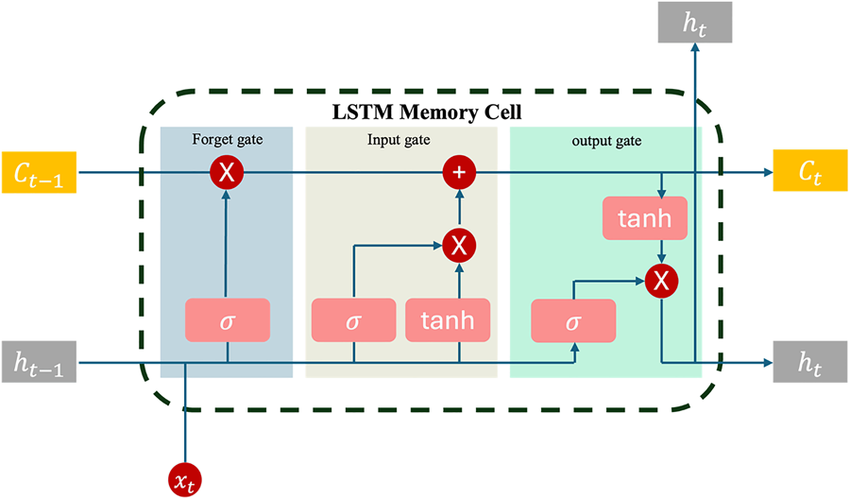
\includegraphics[width=0.7\textwidth]{pics/lstm_memory_cell.png}
    \caption{The architecture of memory cell in LSTM (Source: Dual-transformer deep learning framework \cite{chen2025dual})}
\end{figure}

LSTM can gain or drop information depend on it selection when a state of cell through these gates. This mechanism makes the model performing well in natural language text. It can automatically learn features from raw sequences so that we don't need to construct features like n-gram and TF-IDF. Furthermore, compared to standard Recurrent Neural Networks, LSTMs are specifically designed to address the diminishing gradient issues, which allows them to remember information across longer text spans, a crucial advantage for sentiment analysis tasks.

\subsection{Model Architecture design}
We built the LSTM model with the following steps: processed raw IMDb data into padded integer sequences, added embedding and LSTM layer to extract features, then regularized with dropout, and finally get sentiment classification through a sigmoid activated dense layer.


\begin{figure}[ht]
    \centering
    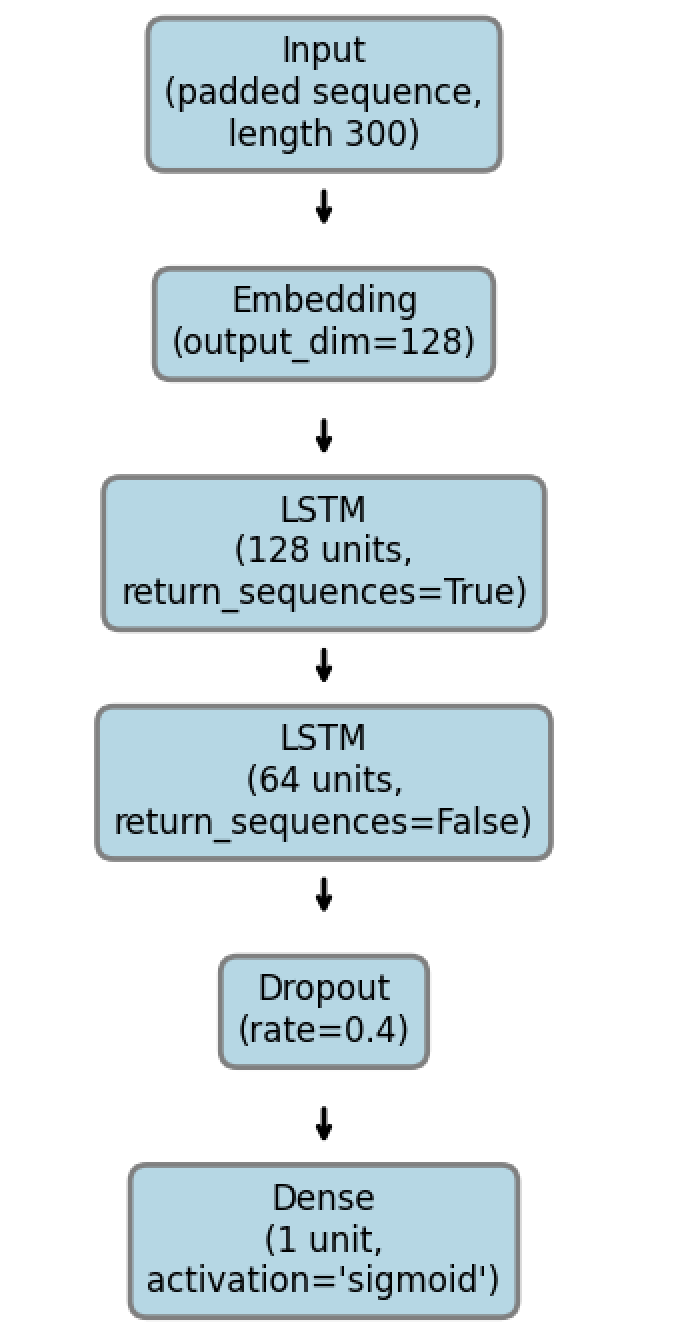
\includegraphics[width=0.3\textwidth]{pics/lstm_architecture_designed.png}
    \caption{The architecture of LSTM}
\end{figure}

\begin{figure}[ht]
    \centering
    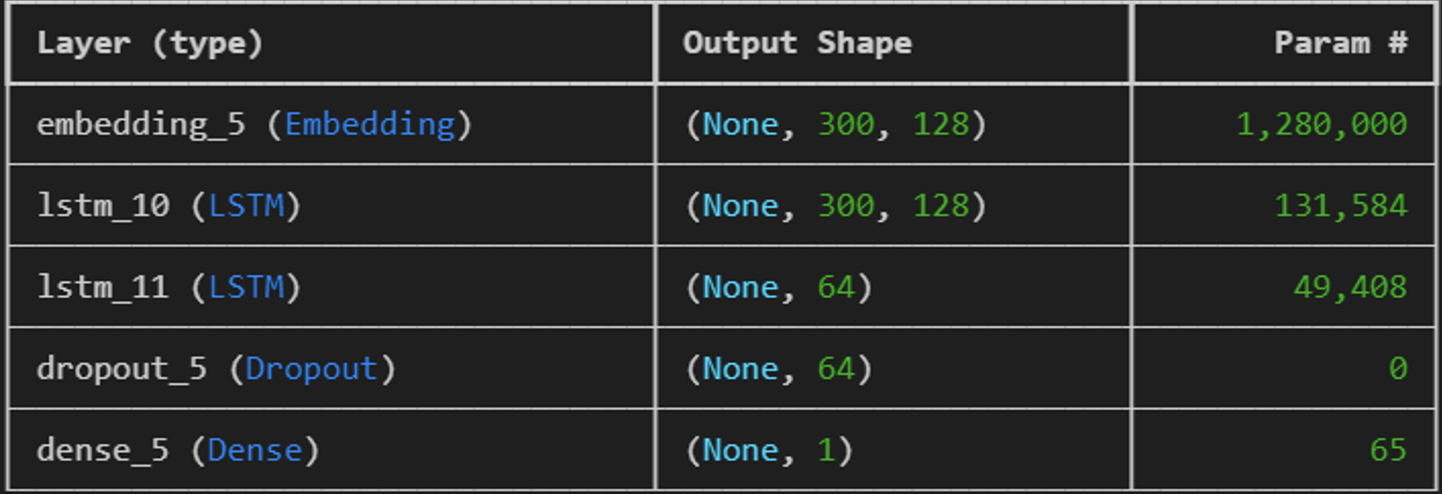
\includegraphics[width=0.6\textwidth]{pics/lstm_model.png}
    \caption{The summary of LSTM}
\end{figure}

The pipeline began with raw IMDb reviews. We proprocessed the data by mapping each word into an integer index and then padding all sequences to a length of 300 tokens. This allowed the data to be trained efficiently in batches. Next we built an Embedding layer, which serves as the input layer. It transforms the integer-encoded vocabulary (limited to the 10,000 most frequent words) into dense, 128-dimensional vectors. This layer is crucial as it learns a meaningful, continuous representation for each word that captures semantic relationships within the vector space.

Next, we stack two LSTM layers to model temporal dependencies in the text. The first LSTM includes 128 hidden units, and it outputs the entire hidden states as a sequence. This seconde LSTM layer has 64 hidden units and outputs only a hidden state from the final time step. This single vector acts as a powerful summary of the entire input sequence, encoding the sentiment of the review.

To reduce the risk of overfitting, dropout layers are added between the LSTM stacks, the drop rate is setting as 0.4, the final dense output layer also added for the same reason. The last layer used a single neuron activated by sigmoid function to predict the probability of the review being positive. The training was performed by using the "Adam" optimization algorithm and Binary cross-entropy (BCE) loss, with model performance evaluated through both accuracy and AUC metrics.

\subsection{Results of LSTM}
After training 50 epochs of our LSTM model, we evaluated it on an unseen test set. Our model got 85.5\% accuracy in the test set, and 88\% of Area Under the ROC Curve (AUC). The results illustrates that our LSTM model has successfully learned sentiment-relevant features from the data.

The classification report showed almost similar value of precision, recall, and F1-scores in positive-negative classes. They all approached around 0.855 which indicates that the model treated both positive and negative reviews with equal effectiveness and no bias.

\begin{figure}[ht]
    \centering
    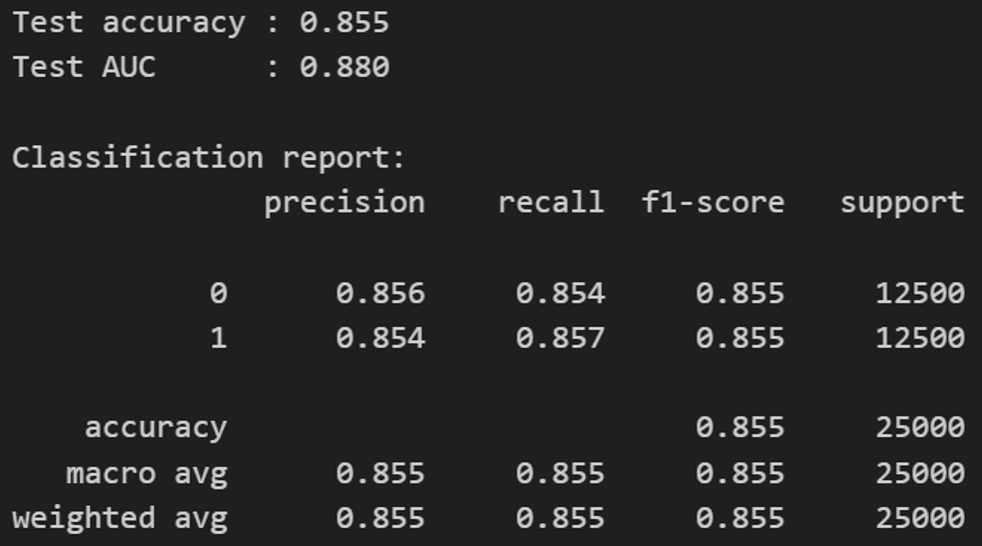
\includegraphics[width=0.6\textwidth]{pics/lstm_report.png}
    \caption{The classification report of LSTM}
\end{figure}

In the confusion matrix, the diagonal values (TN, TP) are much higher than off-diagonal (FP, FN) which shows a high correct rate prediction along the main diagonal versus incorrect predictions. The counts of failed prediction in positives and negatives are very similar, 1827 and 1791 respectively. This balance also supported that the model's errors were not biased towards any one class.

\begin{figure}[ht]
    \centering
    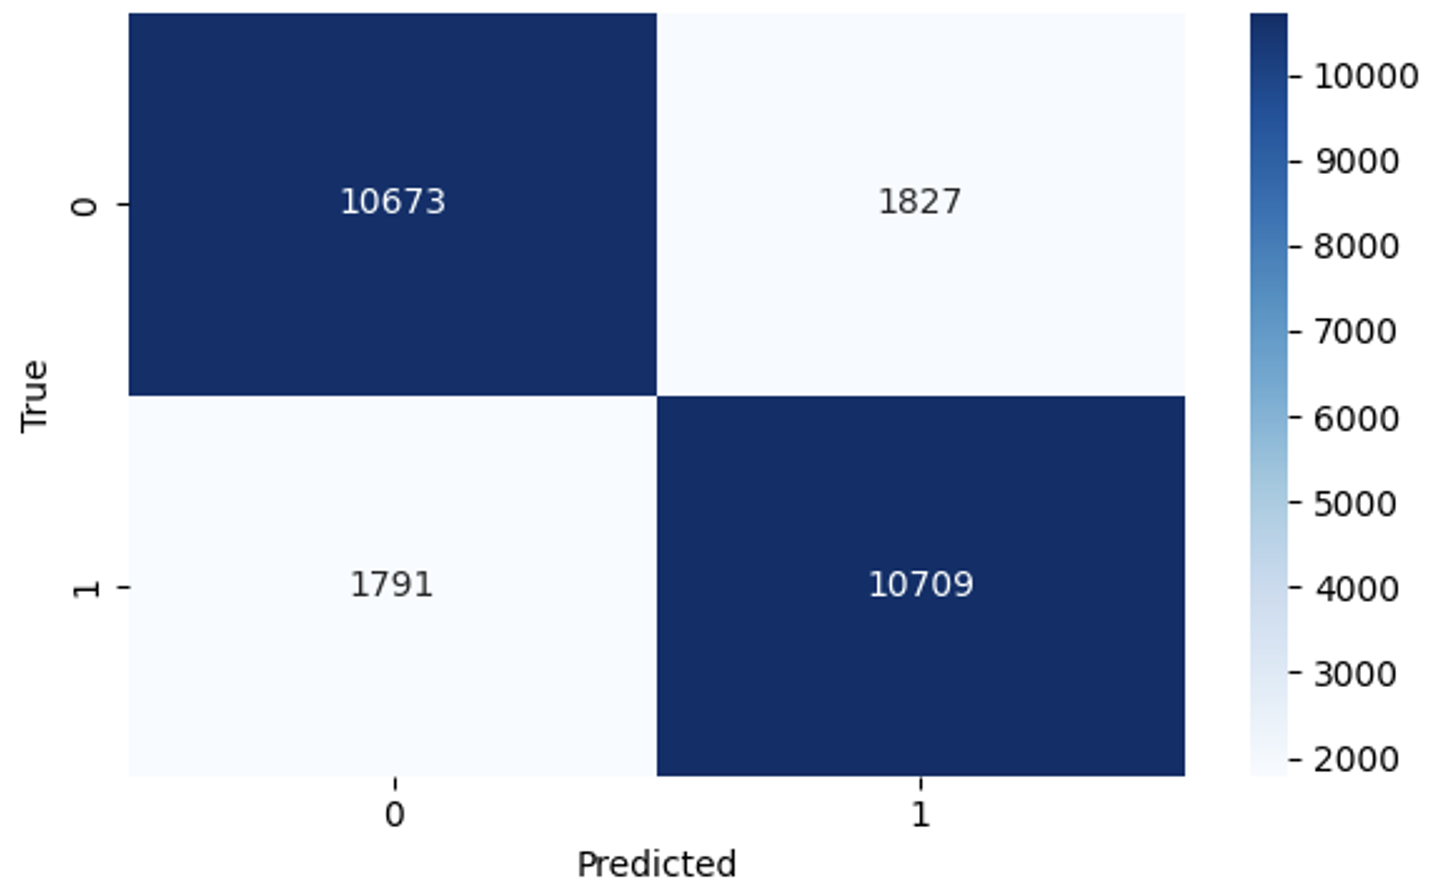
\includegraphics[width=0.6\textwidth]{pics/lstm_metrix.png}
    \caption{The confusion matrix of LSTM}
\end{figure}

\subsection{Optimization on epochs}
In the "Accuracy on epochs" plot, the learning curve of the LSTM model is demonstrated clearly. From the training and validation accuracy curves, it is observed that the validation accuracy stabilizes after the 15th epoch, while the training accuracy continues to rise. This phenomenon suggests a risk of overfitting but can be controlled by regularization and monitoring.

\begin{figure}[ht]
    \centering
    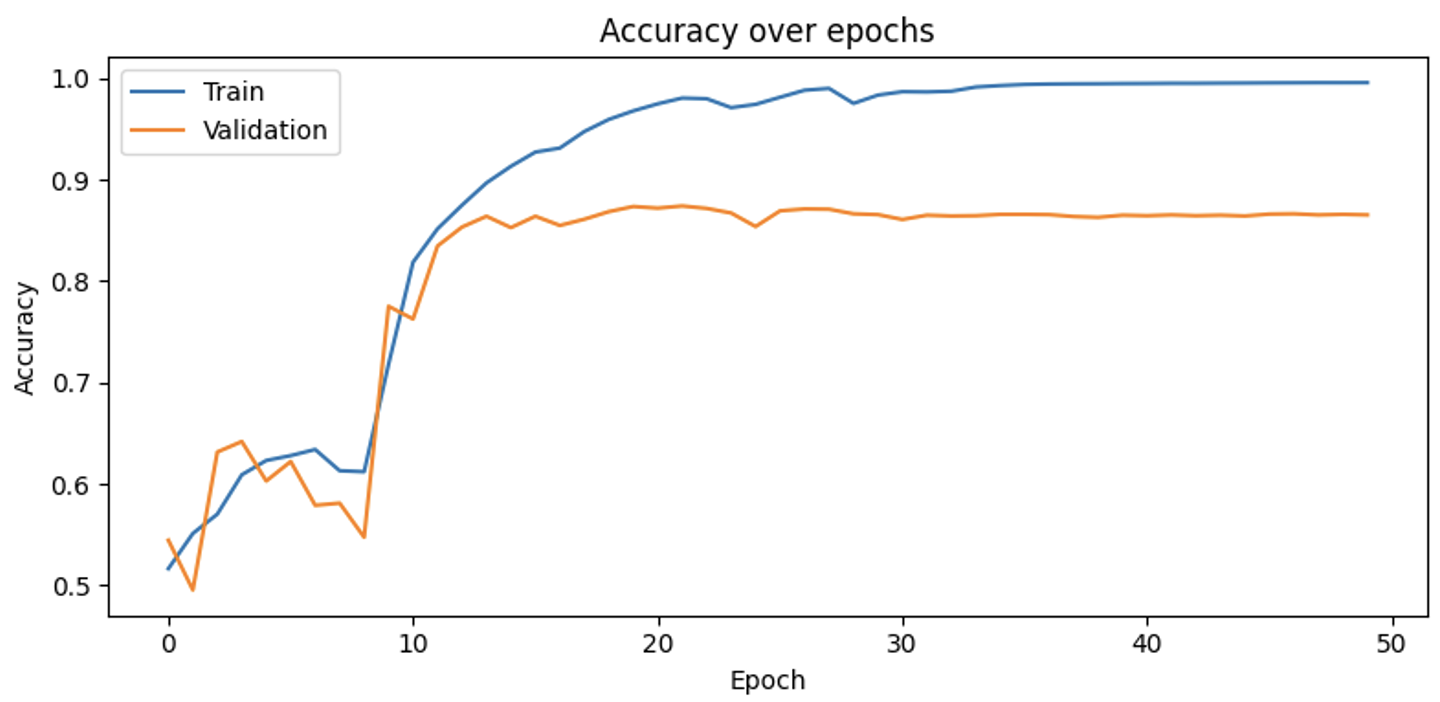
\includegraphics[width=0.6\textwidth]{pics/lstm_accuracy_s.png}
    \caption{Accuracy on epochs of LSTM}
\end{figure}

\subsection{Conclusion}
In summary, LSTM networks offer a powerful and balanced solution for sentiment analysis on the IMDb dataset that outperforms traditional methods and achieves robust and unbiased results. In the future, we can try to make some improvements including the integration of pre-trained word vectors, attention mechanisms, or more sophisticated regularisation techniques, as well as a more formal assessment of the model's statistical significance and generalisation capabilities.





